% =====================================================================
%  《企业筹资风险研究》 —— 海口经济学院毕业论文格式 排版测试稿
%  编译：XeLaTeX 运行两次
% =====================================================================
\documentclass[12pt,a4paper,fontset=windows,UTF8]{ctexart}
\usepackage{hkjjxy-format}
\usepackage{pdfpages}   % 引入学校 Word 模板的封面页与声明页

\cnTitle{企业筹资风险研究}
\cnSubTitle{——以比亚迪股份有限公司为例}
\enTitle{Research on Corporate Financing Risks: A Case Study of BYD Co., Ltd.}

\begin{document}
\pagestyle{plain}

% 封面页 + 声明页：直接使用学校 Word 模板转出的 PDF（front.pdf，共 2 页）
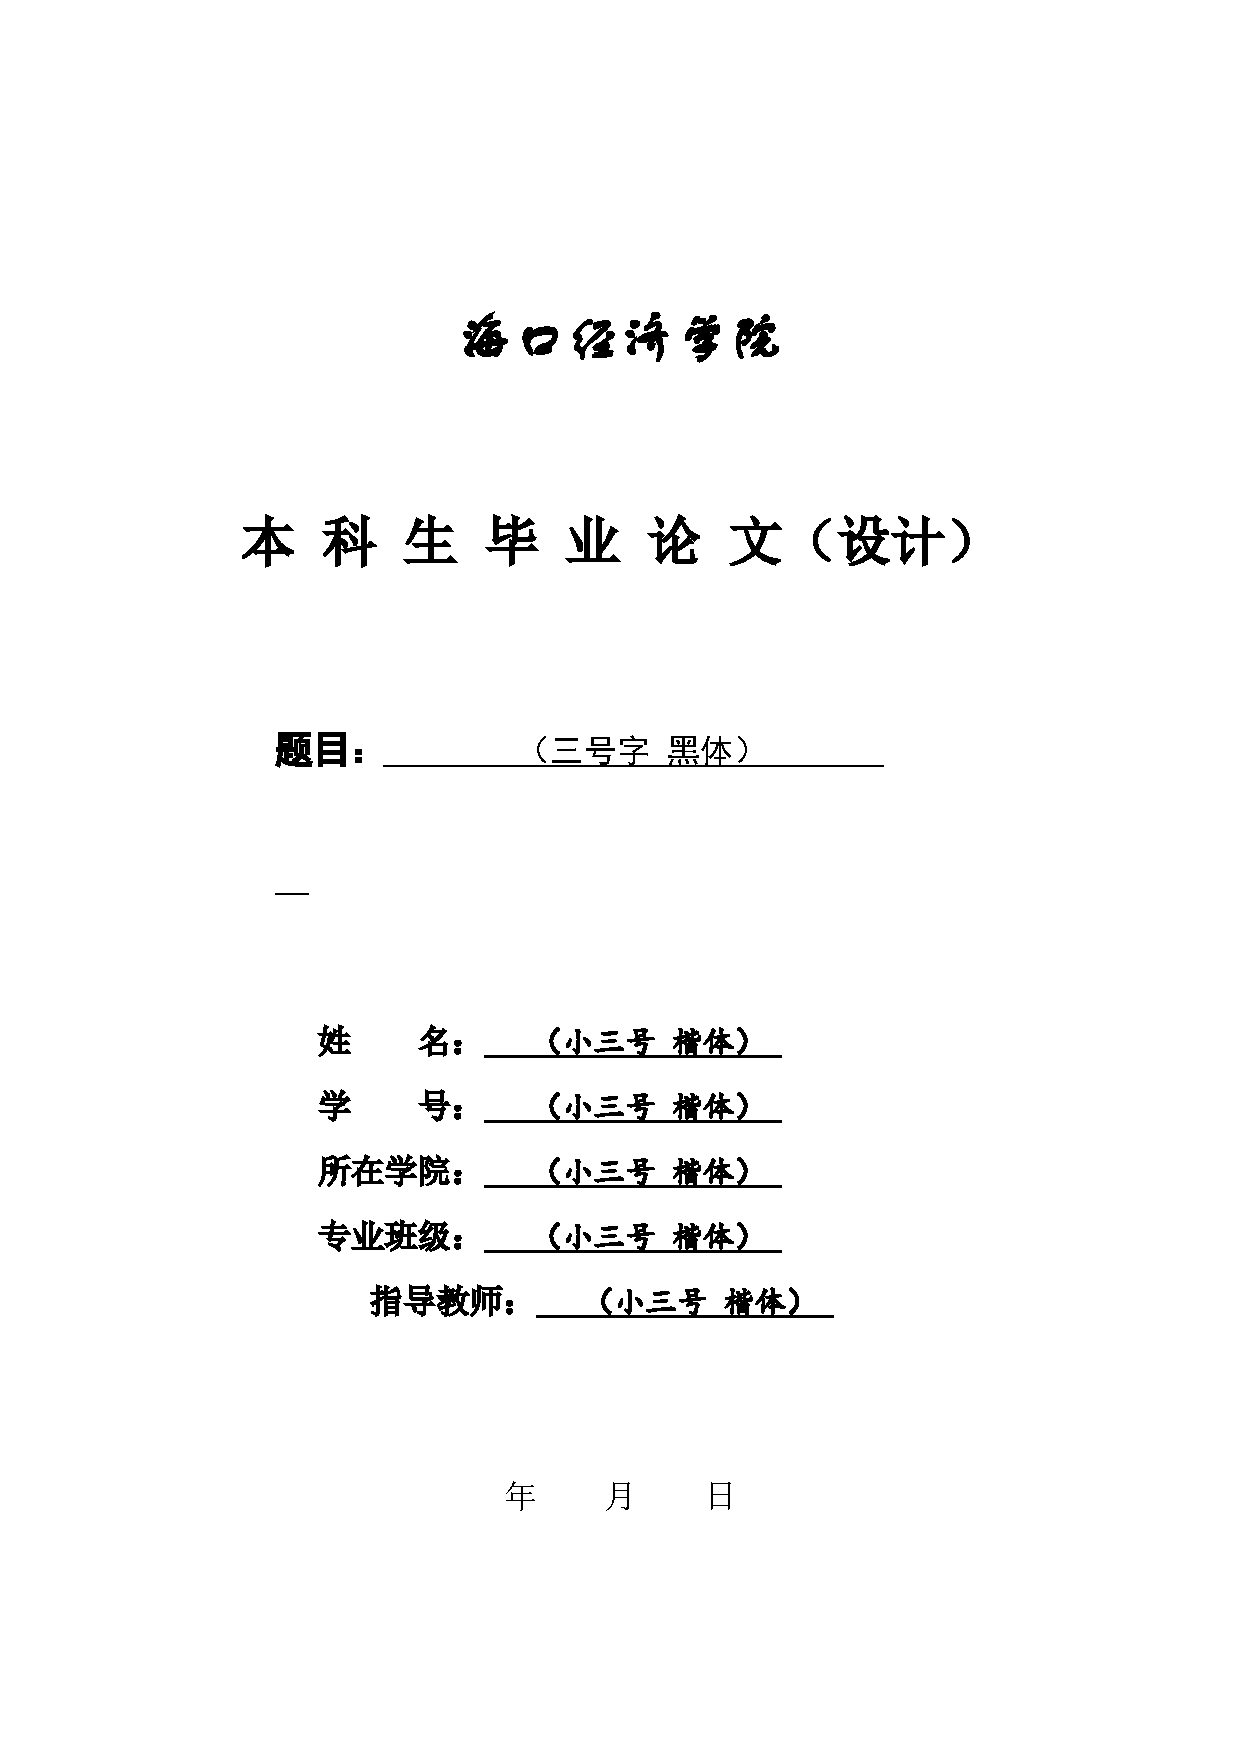
\includepdf[pages=1-2,pagecommand={\thispagestyle{empty}}]{front.pdf}
\tocpage

\setcounter{page}{1}
\pagenumbering{arabic}

\cnTitleBlock

\cnAbstract{%
  在全球新能源汽车产业从“规模博弈”转向“智驾决战”、再转向“本土化深耕”的战略交替期，比亚迪作为行业领头羊，其筹资模式的稳健性对中国汽车工业出海有直接、
  重大的影响，因此本文以2023-2025年为研究窗口，系统、严谨地考察了比亚迪的财务运行体系：即“高增长、重资产、
  高经营杠杆”的结构，指出其产业链垂直整合带来的强势议价能力有利于降低显性财务成本，但是全球化深耕期也伴随着战略性开支脉冲式增长与经营性现金流回笼减速的结构性错配风险。
  更具体地说，2025年比亚迪海外工厂密集上马、智能化研发饱和投入，资本性开支达到高峰，又恰逢国内“价格战”与海外关税壁垒叠加的不利时刻，
  两者叠加对比亚迪内源筹资能力形成极大压力。值得称道的是，本文的实证分析十分清楚地揭示了比亚迪于2025年3月进行巨额H股配售，
  用股权融资主动、充分地缓冲债务压力，由此完成从被动应对筹资风险到主动防御筹资风险的重要转变，也自然、妥帖地引出高成长性企业出海时筹资重心应有的调整方向：
  从传统的“债务规模控制”转向“流动性弹性管理”。因此，比亚迪的案例为中国企业在复杂经贸环境下平衡扩张与安全提供了极其有力、
  极其清晰的实证参考。
}

\cnKeywords{比亚迪；筹资风险；经营杠杆；资本结构}

\enTitleBlock

\enAbstract{%
  In the strategic transition of the global NEV industry from scale competition to intelligent driving and localized manufacturing, BYD’s financing robustness is pivotal to the success of China’s automotive expansion. Focusing on the 2023-2025 window, this study reveals that BYD established a unique financial framework of "high growth and high operating leverage," optimizing explicit costs via vertical integration while simultaneously facing a structural mismatch between impulsive capital expenditures and decelerating cash flow recovery during its globalization phase. As Capex peaked in 2025 due to simultaneous global factory construction and R\&D saturation, domestic price wars and overseas tariff barriers exerted a dual squeeze on internal financing capacity. Empirical analysis highlights that BYD’s massive H-share placement in March 2025 effectively buffered debt pressure through equity financing, marking a transition from reactive mitigation to proactive defense. This case suggests that for high-growth enterprises going global, the financing focus must shift from traditional "debt scale control" to "liquidity elasticity management," providing a scientific reference for balancing expansion velocity with financial security in a volatile global economy.
}

\enKeywords{BYD; Financing Risk; Operating Leverage; Capital Structure}

\newpage

\section*{引言}
\phantomsection
\addcontentsline{toc}{section}{引言}

由于全球气候治理、能源战略转型两者叠加，新能源汽车产业已经成为重塑全球工业格局最有力、最活跃的引擎。因此比亚迪股份有限公司（以下简称“比亚迪”）在2023年以302.4万辆的年度销量问鼎全球新能源汽车销冠，
  也由此让中国自主品牌在汽车百年变革中真正实现在从跟随到引领的跨越式突破。但毋庸讳言，2024—2025年是比亚迪全球化深耕期，
  企业正在从“产品输出”向“产能输出”做系统、有计划的战略重构，海外建厂潮、自有滚装船队建设、智能化技术激进布局都带来了规模空前的资本性开支。
  故而如何在全球化博弈与技术迭代叠加的环境下守住资金链韧性，已然成为比亚迪迈入全球一流企业行列时最直接、最关键的财务命题。

从财务运行逻辑可以十分自然地看到，比亚迪2023-2025年的筹资特征是“高增长、重资产”与“低有息负债、高流动性储备”并存。
  2024年比亚迪541.6亿元的研发投入及全球五大洲制造基地的扩张，都对企业资源调配效率提出了极大的考验，而同年国内市场剧烈的“价格战”对比亚迪利润空间形成直接挤压，
  欧盟、美国等海外市场的关税壁垒又对比亚迪回笼资金构成重大潜在风险，因此2024年比亚迪存在十分明确、也相当庞大的筹资风险敞口。
  故而2025年3月比亚迪进行H股配售募资435亿港元的动作，实质上是其在智驾系统研发、海外扩张两方面不确定性都存在时主动、
  审慎的财务弹性提升及宏观风险对冲安排。

针对比亚迪2023-2025年的筹资风险识别与防控，本文在高度关注企业面临地缘政治紧张局势下复杂的资本结构变化的基础上，
  试图通过对多样化融资方式（经营性负债融资及资本市场股权融资）适度的应用，在促进企业快速发展的同时保障其资金流动性；
  基于对中国新能源企业在出海背景下优化筹资策略、防御系统性财务风险需求的高度关注，以比亚迪为研究对象进行实证分析，
  为其他中国新能源企业提供作战模板和实践路径。

\section{企业筹资风险相关理论基础}

\subsection{企业筹资风险的内涵与分类}

\subsubsection{企业筹资风险}

企业筹资风险，其核心是指企业在筹资活动中由于资金来源结构的不确定性，导致企业丧失偿债能力并使股东收益发生偏离的可能性\textsuperscript{[1]}。
  从本质上审视，筹资风险具有客观存在性与潜在性，伴随企业的融资决策而生。广义的筹资风险不仅包含债务到期无法偿还的信用风险，
  还涉及资本成本波动对企业利润空间的挤压\textsuperscript{[2]}。通过科学的财务治理，这种风险虽然无法完全消除，
  但其发生的概率与影响程度在理论上是具备可控性的。

\subsubsection{筹资风险类型}

在具体分类层面，筹资风险通常可划分为显性风险、隐性风险及结构性风险。显性筹资风险又称收支性风险，主要源于企业经营利润不足以覆盖固定的利息支出，
  表现为终极性的违约；而隐性筹资风险则侧重于反映现金流的“时间差”矛盾，即即便企业账面盈利，若资产流动性不足以匹配到期负债，
  仍会诱发临时性支付危机。此外，结构性风险则聚焦于债务期限结构与资本构成比例，如长短期债务比例失调所引发的财务韧性下降。

\subsection{企业筹资风险的成因}

\subsubsection{企业筹资风险的内部原因}

从企业内部微观治理维度来看，筹资风险的生成机理首先源于资本结构的失衡。根据财务杠杆理论，当企业负债规模过大时，
  财务杠杆系数（DFL）会显著升高，这虽然在经济上行期能放大股东回报，但一旦息税前利润发生波动，高杠杆将剧烈放大收益的下滑幅度，
  产生负杠杆效应\textsuperscript{[3]}。与此同时，债务结构错配也是关键诱因，过度依赖流动负债来支持长期资产投入，
  会使企业陷入借新还旧的被动局面\textsuperscript{[3]}。此外，管理层的决策偏差同样不容忽视，
  在行业红利期产生的过度自信往往会导致资本开支计划脱离实际资金承受能力，进而埋下风险隐患\textsuperscript{[4]}。

\subsubsection{企业筹资风险的外部原因}

外部环境的变化则构成了筹资风险的宏观成因。金融市场的波动，如银行信贷政策的收紧、市场基准利率的上行以及汇率的剧烈变动，
  会直接推高企业的融资成本\textsuperscript{[5]}，对于进行全球化布局的企业而言，外币债务风险尤为显著\textsuperscript{[6]}。
  同时，新能源汽车行业作为政策敏感型产业，行业政策的调整如补贴退坡等会直接挤压净利润\textsuperscript{[7]}，
  削弱内源筹资能力。在宏观经济周期下行阶段，市场需求的疲软导致回款减速，资产变现能力弱化，这种外部压力的叠加会进一步放大企业的偿债压力\textsuperscript{[8]}。

\subsection{企业筹资风险的控制策略}

针对识别出的筹资风险，学术界与实务界构建了一套系统性的控制策略体系。首先是风险规避策略，通过详尽的可行性论证，
  主动放弃成本过高或回报期过长、可能危及现金流安全的筹资项目\textsuperscript{[9]}。其次是风险降低策略，
  通过优化负债期限结构、延长长期债务占比，并实施紧缩的信用政策以加快资金回笼\textsuperscript{[2]}。
  此外，风险转移策略利用远期结售汇等金融工具对冲汇率波动，或通过应收账款保理将信用风险转嫁至金融机构\textsuperscript{[10]}。
  最后，风险承担策略通过建立财务储备金制度，构建财务缓冲带以应对突发性的流动性需求。

构建动态预警系统是现代财务管理策略实施中十分明确、重要的环节，而定量评价模型Altman的Z-Score模型及改进的F分数模型都很好地利用了资产负债率、
  现金流动负债比诸种财务指标来评价企业财务健康度。更难得的是，F分数模型引入了经营现金流量指标，因此在评价重资产、
  高扩张企业的财务韧性时要远比传统模型准确。企业可借助信息技术设定关键财务指标的红线阈值，真正将风险从被动应对转为主动预警\textsuperscript{[2]}。

\subsection{汽车行业的筹资风险特征}

新能源汽车行业有十分明确、可辨识的技术密集型、重资产型特性，因此其筹资风险逻辑有极其鲜明的特点：由于技术更新换代极快，
  企业要保持竞争优势就必须持续投入大量研发资金，故而企业在扩张期常遇到“增产不增现”的悖论。又因为大规模工厂建设及全球供应链布局都属于长周期投资，
  资金回收期极长，故企业在形成规模效应以前必然高度依赖外部举债。二者叠加之下，技术创新的不确定性与资本开支的刚性需求彼此纠缠，
  也自然地形成了新能源汽车行业特有的财务脆弱性。

此外，头部车企在供应链金融中所呈现的“双刃剑”效应是分析起点。头部车企以强势议价能力压低供应商账期，因此能降低显性财务成本，
  这种模式虽然降低了显性的财务成本，但也隐含着深刻的隐性风险，依托产业链互信建立起来的资金链极有可能发生连锁反应，
  进而爆发系统性支付危机。为此，研究比亚迪等企业在2023—2025年战略跨越期筹资风险具有极强的现实意义。

\section{比亚迪筹资风险识别}

\subsection{比亚迪概况}

比亚迪成立于1995年，初创时期深耕充电电池领域，凭借成本控制与技术迭代迅速跻身全球电池供应商第一梯队。2003年，
  比亚迪通过收购西安秦川汽车正式跨界进入整车制造领域，这一动作拉开了其长达二十载的“垂直整合”序幕。时至今日，比亚迪已演变为横跨汽车、
  轨道交通、新能源及电子四大产业的跨国巨头，不仅蝉联全球新能源汽车销量桂冠，更构建了从矿产资源开发、动力电池研发（刀片电池）到半导体芯片设计（比亚迪半导体）的闭环生态系统。

比亚迪的核心竞争力在于其极端的“垂直整合”模式。这种模式在供应链动荡时期赋予了企业极强的生存韧性，使其能够规避外部零部件短缺的冲击。
  进入2023—2025年的战略转型深水区，比亚迪的战略焦点已由早期的“产能占位”转向“智驾突围”。通过发布“天神之眼”高阶智驾系统及整车智能策略，
  比亚迪试图在保持硬件规模优势的同时，重塑软件算法的溢价能力。这种由硬件制造向“硬软一体”跨越的逻辑，构成了其近年来大规模资本开支与研发饥渴的战略诱因。

在财务运行层面，比亚迪表现出一种异于传统车企的“信用驱动型”特征。由于其在产业链中处于绝对主导地位，比亚迪能够通过海量的无息应付账款替代有息融资，
  从而在维持高资产负债率的同时，有效压降显性利息成本。这种独特的财务底色，使其具备了“以规模博时间”的博弈筹码。
  然而，随着全球化出海进程中海外基地（如匈牙利、巴西工厂）的重资产投入加大，这种依赖内源性信用杠杆的模式正面临跨市场、
  跨周期的动态压力测试。

\subsection{比亚迪筹资风险的识别}

风险识别是筹资风险管理的首要环节，因此从对比亚迪2023—2025年财务数据的分析中可以发现其筹资风险具有明确的“高杠杆、
  低压力”特征：一方面，资产负债率长期处于70\% 以上的高位，但是其中八成以上系无息应付账款构成，故显性偿债压力实际受控。
  另一方面，2025年海外建厂、智能化研发都进入资金投入高峰，流动比率的波动及有息负债的阶段性激增已经成为新的风险识别焦点。
  下文将从偿债指标的演变与债务结构的两个维度，对比亚迪 2023-2025 年的筹资风险进行量化剖析。

\subsubsection{偿债能力风险识别}

从资本结构的角度可以看到，比亚迪资产负债率近三年间持续地下降：2023年末为77.86\%，当时处在行业较高水平，
  2024年末降为74.64\%，到2025年又降为70.74\%。虽然目前资产负债率绝对值仍然较高，但是比亚迪负债的绝大部分为无息经营性负债，
  非高利息的有息负债，因此比亚迪的实际财务风险处于极好的控制之中。

从动态趋势来看，比亚迪资产负债率呈现逐年下降态势，资本结构持续优化，具体数据 如表~\ref{tab:t1} 所示。

\begin{thesTab}[htbp]{资产负债率分析表\label{tab:t1}}{数据来源：2023-2025年比亚迪年度报告}
\begin{tabularx}{0.86\linewidth}{X c c c}
  \toprule
  财务指标 & 2023 年 & 2024 年 & 2025 年 \\
  \midrule
  资产总额 (亿元) & 6,795.50 & 7,833.60 & 8,837.30 \\
  负债总额 (亿元) & 5,290.90 & 5,846.70 & 6,251.90 \\
  资产负债率 & 77.86\% & 74.64\% & 70.74\% \\
  \bottomrule
\end{tabularx}
\end{thesTab}

从短期偿债能力的角度，流动比率由2023年的0.67上升到2025年三季度的0.87，速动比率也从0.44升到0.56，
  虽然二者尚未达到传统上所认为的2.0及1.0的安全标准，但是其中必然有汽车制造业存货规模巨大、预收账款较多的行业特性影响。
  因此比亚迪短期偿债弹性正在良性修复。

从静态时点来看，比亚迪短期偿债指标虽持续改善，但仍低于传统安全线水平，具体数据 如表~\ref{tab:t2} 所示。

\begin{thesTab}[htbp]{短期偿债指标分析表\label{tab:t2}}{数据来源：2023-2025年比亚迪年度报告}
\begin{tabularx}{0.86\linewidth}{X c c c}
  \toprule
  财务指标 & 2023 年 & 2024 年 & 2025 年 \\
  \midrule
  流动比率 & 0.67 & 0.75 & 0.79 \\
  速动比率 & 0.44 & 0.47 & 0.42 \\
  \bottomrule
\end{tabularx}
\end{thesTab}

\subsubsection{债务结构风险识别}

从比亚迪债务结构可以归纳出其的特征：“有息负债极低，经营性负债极高”。即2023、2024年比亚迪有息负债规模一直在200亿～300亿的低位，
  占总负债的比例不足5\%，但2025年为配合全球工厂建设及智能化研发的需要，公司有息负债规模于第三季度末增至814.9亿元，
  所筹资金主要来自银行借款及发行科技创新债券。

由于比亚迪2024年末无息负债（应付账款及合同负债）已达2854亿元，故从正反两方面来评价比亚迪利用供应链议价能力取得无息融资的做法：
  即其有利于降低财务成本，但是也带来了若销量断崖式下滑或供应链信用受损，巨额应付款项就会变成重大现金流回款风险的结构性风险。

进一步拆解负债内部结构，可以清晰看到有息负债与经营性负债的分化走势，具体数据 如表~\ref{tab:t3} 所示。

\begin{thesTab}[htbp]{债务结构分析表\label{tab:t3}}{数据来源：2023-2025年比亚迪年度报告}
\begin{tabularx}{0.86\linewidth}{X c c c}
  \toprule
  指标 (单位：亿元) & 2023 年 & 2024 年 & 2025 年 \\
  \midrule
  短期借款 & 183.2 & 121 & 384.8 \\
  长期借款 & 119.8 & 82.6 & 607.1 \\
  应付债券 & 0 & 0 & 50 \\
  租赁负债 & 88.5 & 98.8 & 86.2 \\
  有息负债合计 & 391.5 & 302.4 & 1,128.10 \\
  应付账款 & 1,944.30 & 2,416.40 & 1,867.40 \\
  经营性负债 & 4,900.00 & 5,545.00 & 5,124.00 \\
  有息负债占比 & 7.39\% & 5.17\% & 18.04\% \\
  \bottomrule
\end{tabularx}
\end{thesTab}

\subsubsection{动态筹资风险识别}

\paragraph*{（1）财务杠杆系数（DFL）}

通过对财务杠杆系数的测算，可以量化评价筹资风险对企业利润的影响程度。根据公式DFL = EBIT/(EBIT - I)，
  2023 年比亚迪的息税前利润（EBIT）约 391亿元，利息支出为 18.3 亿元，测算得 DFL 约为 1.049。
  2024 年 EBIT 增至 517.7亿元，利息支出约为 20.9 亿元，DFL 降至 1.042。较低的 DFL 指标表明，
  虽然比亚迪负债总额巨大，但由于利息支出相对利润规模极小，财务杠杆并未产生过度的风险放大效应，企业具备极强的利润抗压能力。

通过上述指标测算，比亚迪财务杠杆水平及其保障程度 如表~\ref{tab:t4} 所示。

\begin{thesTab}[htbp]{财务杠杆系数分析表\label{tab:t4}}{数据来源：2023-2025年比亚迪年度报告}
\begin{tabularx}{0.86\linewidth}{X c c c}
  \toprule
  财务指标 & 2023 年 & 2024 年 & 2025 年 \\
  \midrule
  息税前利润 EBIT (亿元) & 391 & 517.7 & 423 \\
  利息支出 (亿元) & 18.3 & 20.9 & 25.5 \\
  DFL & 1.049 & 1.042 & 1.064 \\
  利息保障倍数 & 21.39 & 24.73 & 16.58 \\
  经营现金流 / 流动负债 & 37.40\% & 26.90\% & 12.60\% \\
  流动比率 & 0.67 & 0.75 & 0.79 \\
  \bottomrule
\end{tabularx}
\end{thesTab}

\paragraph*{（2）现金流分析}

从对比亚迪2023-2025年现金流量表所做的系统、严谨的分析中，可以出其筹资风险的成因具有典型的“扩张驱动型”特征：
  2024年比亚迪经营性现金流净额为1334.5亿元，基本足以覆盖当年1290.8亿元的投资性现金支出。但2025年前三季度海外工厂（泰国、
  匈牙利、巴西等）全部投产，又恰逢智驾系统“天神之眼”研发高速扩张，故2025年投资性现金流出已达1974.63亿元，
  大大超过同期经营现金流回笼速度。这种资本性开支的季节性与阶段性错配，是导致 2025 年企业融资需求激增、筹资风险敞口扩大的直接原因。

从现金流量的分类结构观察，比亚迪资金运作的整体特征 如表~\ref{tab:t5} 所示。

\begin{thesTab}[htbp]{现金流分析表\label{tab:t5}}{数据来源：2023-2025年比亚迪年度报告}
\begin{tabularx}{0.86\linewidth}{X c c c}
  \toprule
  现金流量财务指标 & 2023 年度 & 2024 年度 & 2025 年度 \\
  \midrule
  经营活动产生的现金流量净额 & 1,697.25 & 1,334.54 & 591.36 \\
  投资活动产生的现金流量净额 & -1,256.64 & -1,290.82 & -1,974.63 \\
  筹资活动产生的现金流量净额 & 128.17 & -102.68 & 1,046.14 \\
  \bottomrule
\end{tabularx}
\end{thesTab}

\section{比亚迪筹资风险成因分析}

\subsection{偿债风险成因分析}

比亚迪产能超常规扩张与资产固化引发的偿债风险。比亚迪资产负债率高居 70\% 以上且流动比率持续低迷，其根本成因在于企业正处于从产品输出向产能输出转型的资产阵痛期。
  2025 年三季度末，比亚迪在建工程余额激增至 487.9 亿元，这种跨越式增长背后的直接推手是泰国、巴西、匈牙利等全球制造基地的同时开工。

这种重资产扩张不仅是厂房的堆砌，更包含了如开拓者 1 号等自有船队的组建，旨在构筑物流闭环。然而，从财务逻辑审视，
  这些投入具有极强的资产专用性，导致大量流动资金被迅速锁死在回收周期极长的固定设施中。当重资产企业的债务规模接近临界点时，
  其财务弹性会发生边际递减。由于核心资产已被大规模用于抵押以支撑信贷，比亚迪在面临突发流动性需求时，实际上缺乏足够的变现空间。
  这种产能抢跑导致的资产固化，正是其偿债风险长期处于高位的物理原罪。

\subsection{债务结构风险分析}

债务结构中经营性负债占比超过八成，源于比亚迪对自身产业链话语权的极限变现。截至 2024 年末，比亚迪通过无息占用供应商资金形成了高达 2854 亿元的隐性筹资。
  这种融资模式的成因在于其长期奉行的电比油低定价策略所带来的规模红利。

然而，这一结构的危险性在于它极度依赖终端市场的利润厚度。2025 年上半年，由于国内价格战异常惨烈，比亚迪为了捍卫市场份额，
  不得不牺牲利润空间，导致汽车业务毛利率由 18.78\% 降至 18.01\%。利润空间的萎缩直接削弱了企业的造血功能，
  使得原本作为低成本融资工具的应付账款，变成了随时可能因为销量放缓或信用波动而集体爆发的债务炸弹。这种将筹资安全建立在供应商容忍度之上的逻辑，
  是其债务结构性风险不断累积的根本诱因

\subsection{动态筹资风险分析}

动态筹资压力在 2025 年的集中爆发，本质上是战略投入强度与经营回款节奏的错位震荡。2025 年有息负债从 300 亿规模跳涨至 814.9 亿元，
  其直接诱因是企业进入了智能化下半场及物流闭环建设的资本开支高峰。

成因在于天神之眼高阶智驾系统的研发投入具有极强的刚性与不可逆性。2025 年前三季度，比亚迪投资性现金流出高达 1974.63 亿元，
  这种支出强度远超同期经营性现金流的回笼速度。虽然 2025 年 3 月通过向中东主权基金等配售 H 股拿到了 433.8 亿港元的头寸，
  但这笔资金在五大洲产能落地及研发烧钱的背景下，仅能起到阶段性对冲作用。加之三季度出现的 15 亿元汇兑损益进一步稀释了利润，
  这种由全球化野心驱动的资本饥渴，导致了 DFL 指标在利润波动时的敏感性显著增强，揭示了动态筹资风险在战略扩张节点上的必然性。

\section{比亚迪股份有限公司筹资风险的控制策略建议}

针对前文识别的筹资风险特征及其生成的底层原因，比亚迪应从提升财务弹性、优化信用杠杆及平抑跨境波动三个维度，提出系统性的筹资风险控制对策。

\subsection{针对偿债风险的资产流动性提升与权益资本优化}

\subsubsection{推进核心业务分拆上市以夯实权益底座}

公司应充分利用当前资本市场对新能源产业链的高估值溢价，加快弗迪电池、比亚迪半导体等成熟业务板块的独立 IPO 进程。
  通过引入全球战略投资者，不仅可以直接获取低成本的权益性资本，切实降低资产负债率，更能通过信号传递效应释放企业垂直整合的潜在价值。
  这种做法从根本上改变了单纯依靠母公司负债支撑海外工厂建设的局面，实现了风险在子业务单元层面的有效分散。

\subsubsection{引入绿色金融工具与 AI 决策中枢的实时监测}

比亚迪应将 ESG 表现转化为融资溢价，发行与碳减排目标挂钩的绿色科创债，利用低息长效资金替代传统的高成本信贷。
  同时，基于现有的 IT 优势，升级财务 AI 决策系统，将泰国、匈牙利等地的海外在建工程进度与实时筹资缺口进行分钟级对齐。
  通过模拟“价格战持续”或“关税升级”等极端情境下的压力测试，确保企业在偿债高峰期到来前，即能启动储备式筹资预案。

\subsection{针对债务结构风险的期限结构重构与供应链信用共生}

针对流动负债占比过高及过度依赖供应商账期的结构性隐患，比亚迪需实现从“占压资金”向“管理信用”的战略转型。

\subsubsection{遵循期限匹配原则实施长债置换策略}

针对天神之眼高阶智驾研发及开拓者 1 号自有船队等长周期项目，比亚迪应严格执行期限匹配原则，大幅压缩短期银行贷款规模。
  转而发行五年期及以上的定向债券，利用长期稳定的资金回笼预期来覆盖技术研发与物流建设的投入周期。这种债权期限的拉长，
  能有效对冲短期负债在金融环境收缩时可能诱发的流动性枯竭风险。

\subsubsection{搭建区块链信用平台防范信用反噬}

针对数千亿规模的应付账款，比亚迪应推广基于区块链技术的信用流转平台，实施反向保理。通过将自身的优质信用凭证数字化并向二三级供应商传导，
  使其能够以较低成本获取银行贴现，从而在不缩短比亚迪实际账期的前提下，缓解供应商的流动性焦虑。这种“信用共生”模式能有效化解因销量波动或行业环境恶化时，
  庞大经营杠杆可能触发的集体挤兑或信用崩塌。

\subsection{针对动态筹资压力的跨境对冲与战略支出基金化}

针对战略跨越期资本性开支与经营现金回笼的逻辑错位，比亚迪需构建跨市场、跨周期的资金缓冲矩阵。

\subsubsection{实施自然套期与属地融资匹配机制}

为了平抑 2025 年出现的巨额汇兑损益及资金被动锁死风险，比亚迪应在海外核心市场推行属地融资策略。在泰国、巴西等制造基地直接筹集当地货币债务，
  用于支付当地工厂建设与采购支出。利用海外销售形成的本币收入偿还当地负债，实现经营现金流与筹资现金流在币种上的自动对冲，
  从源头上锁定跨境筹资的波动成本。

\subsubsection{建立研发里程碑挂钩的结构化产业基金}

面对智能化下半场饱和式研发的资金渴求，比亚迪宜联合政府引导基金、主权财富基金等建立结构化产业投资基金。将“天神之眼”等高风险、
  高投入项目进行项目化运作，根据研发里程碑的达成情况动态注入资金。这种做法能显著降低 DFL 指标对企业整体利润的干扰，
  将单一企业的筹资压力转化为产业协同的共担机制，确保在全球化决战期拥有稳健的资本韧性。

\section{结论}

通过对比亚迪股份有限公司 2023—2025 年战略转型期筹资风险的系统性审视，本文得出如下核心结论：

第一，比亚迪在问鼎全球新能源销冠的过程中，构建了一种极其独特的筹资逻辑，即基于全产业链垂直整合能力的“信用杠杆模式”。
  这种模式的本质是利用极强的议价红利，以规模化的无息经营性负债替代高成本的有息债务。然而，分析发现，随着全球化深耕与智能化研发进入决战期，
  这种模式正面临风险边界的收缩。地缘政治引发的海外资金锁死与国内价格战导致的利润空间收窄，使得这种过度依赖单一供应链信用的融资结构显现出明显的防御弱点，
  极易在外部环境震荡下诱发信用反噬。

第二，比亚迪当前的筹资风险具有显著的“扩张节奏与现金流错位”特征。2025 年在建工程的爆发式增长与智驾系统研发的饱和式投入，
  属于典型的战略前置性支出。这种“脉冲式”投入与海外关税壁垒、供应链回收周期之间形成了严重的时间跨度错配。虽然比亚迪账面现金充沛，
  展现了极强的风险耐受力，但重资产模式下财务弹性的边际递减效应依然客观存在。这种“以未来换规模”的博弈，使得企业在面临宏观震荡时，
  通过变现资产来对冲压力的弹性空间被动收窄。

第三，比亚迪在 2025 年的一系列风险对冲动作，特别是 3 月实施的 H 股配售融资，标志着其筹资战略从“被动补缺”向“战略性防御冗余”的质变。
  这一动作通过股权稀释有效对冲了债务依赖，为智能化研发预留了充足的流动性头寸，堪称重资产企业在资本波动期提升财务韧性的实证范式。

综上所述，高成长性企业的筹资风险管理已不再是简单的债务规模控制，而是应上升至“流动性弹性动态博弈”的战略高度。
  比亚迪的案例昭示，中国企业出海必须构建跨市场、多节点的财务护城河。未来，比亚迪宜继续推进全球融资体系的属地化建设，
  主动稀释对单一供应端杠杆的依赖，并通过智能化溢价提升内源造血功能，在保持扩张进攻性的同时，实现财务安全性与战略雄心的深度对冲。

% =====================================================================
% 参考文献（距正文空三行，不另起一页）
% =====================================================================
\vspace*{3\baselineskip}
\unnumsec{参考文献}

\begin{thesref}
  \item 曹雪. 企业筹资方式和筹资风险探析[J]. 中国集体经济, 2025(11): 77-80.
  \item 左晓曼. 现金流视角下比亚迪汽车财务风险控制研究[D]. 河北经贸大学, 2025.
  \item 戴雨薇. 比亚迪财务风险管理研究[D]. 长江大学, 2025.
  \item 徐嘉蔚.哔哩哔哩公司筹资风险与控制措施[J].投资与合作, 2024(10): 139-141.
  \item 王明月. 企业财务风险管理中的筹资风险分析及控制策略[J]. 纳税, 2024, 18(34): 58-60.
  \item 薛建. 快消品A企业筹资风险识别及其防范研究[D]. 山西财经大学, 2023.
  \item 刘小梅. 互联网金融筹资风险研究[J]. 全国流通经济, 2022(11): 127-129.
  \item 林泽华. 小鹏汽车公司筹资风险管理研究[D]. 吉林大学, 2022.
  \item 冯军. 企业债务融资及其偿债能力与筹资风险分析[J]. 纳税, 2019, 13(14): 212, 214.
  \item 岳云娇. J公司筹资风险管理研究[D]. 天津农学院, 2018.
  \item Othman M, Nagina R, Saini A. Predictive Analysis of Financial Distress in Pharma Sector: A Quantitative Approach using Altman’s Z-Score Model[J]. International Journal of Religion, 2024.
  \item Challoumis C. How AI insights are revolutionizing financial strategies for enterprises[C]XIV International Scientific Conference. 2024: 108-140.
  \item Andronie M, Iatagan M, Uță C, et al. Big data management algorithms in artificial Internet of Things-based fintech[J]. Oeconomia Copernicana, 2023, 14(3): 769-793.
  \item MA Z, WANG X, HAO Y. Development and application of a hybrid forecasting framework based on improved extreme learning machine for enterprise financing risk[J]. Expert Systems with Applications, 2023, 215: 119373.
  \item HU X, MUWAFAK B M. Mathematical modelling of enterprise financial risk assessment based on risk conduction model[J]. Applied Mathematics and Nonlinear Sciences, 2022, 7(1): 591-600.
\end{thesref}

% =====================================================================
% 致谢（原文未提供，请补写；距参考文献空三行，不另起一页）
% =====================================================================
\vspace*{3\baselineskip}
\unnumsec{致谢}

（原文未提供致谢内容，请在此补写。）

\end{document}